\documentclass[12pt, a4paper]{report}

\usepackage[utf8]{inputenc}
\usepackage[english]{babel}
\usepackage{setspace}
\usepackage{amsmath,amssymb,amsthm,mathtools,cases,bm}

\theoremstyle{definition}
\newtheorem{Example}{Example}
\newtheorem{Theorem}{Theorem}
\newtheorem{ToDo}{ToDo}

\usepackage{varioref,hyperref,cleveref}
\usepackage[pdftex]{graphicx}
\usepackage{caption,float,epstopdf,subfig}

\renewcommand{\thefigure}{\arabic{figure}}

\usepackage{listings}
\usepackage[dvipsnames]{xcolor}

\lstset{language=[ISO]C++,
				backgroundcolor = \color{blue!5!white},
				aboveskip=10pt, belowskip=10pt,
				numbers=left, numberstyle=\tiny,
				tabsize=2,
				breaklines=true,
				basicstyle=\small\ttfamily,
				keywordstyle = \color{blue!50!cyan}\bfseries,
				commentstyle = \color{darkgray!90},
				stringstyle = \color{OliveGreen},
				morecomment=[l][\color{violet!90!black}]{\#},
				identifierstyle=\color{blue!25!black}
				literate=
				{á}{{\'a}}1 {é}{{\'e}}1 {í}{{\'i}}1 {ó}{{\'o}}1 {ú}{{\'u}}1
				{Á}{{\'A}}1 {É}{{\'E}}1 {Í}{{\'I}}1 {Ó}{{\'O}}1 {Ú}{{\'U}}1
				{à}{{\`a}}1 {è}{{\`e}}1 {ì}{{\`i}}1 {ò}{{\`o}}1 {ù}{{\`u}}1
				{À}{{\`A}}1 {È}{{\'E}}1 {Ì}{{\`I}}1 {Ò}{{\`O}}1 {Ù}{{\`U}}1}

\renewcommand*{\thefootnote}{\fnsymbol{footnote}} 
	
\title{\textbf{Deep Learning for PDEs}\\
			\large Report of the joint APSC-NAPDE courses project}
\author{Paolo Joseph Baioni\footnote{\href{mailto:paolojoseph.baioni@mail.polimi.it}{paolojoseph.baioni@mail.polimi.it}}}
\date{\today}

\begin{document}

	
\maketitle

\renewcommand*{\thefootnote}{\arabic{footnote}}
\setcounter{footnote}{0}

	
%%%%%%%%%%%%%%%%%%%%%%%%%%%%%%%%%%%%%%%%%%%%%%%%%%%%%%%%%%%%%%%%%%%%%%%%
%%%%%%%%%%%%%%%%%%%%%%%%%%%%%%%%%%%%%%%%%%%%%%%%%%%%%%%%%%%%%%%%%%%%%%%%	
	

%\chapter*{Acknowledgements}


%%%%%%%%%%%%%%%%%%%%%%%%%%%%%%%%%%%%%%%%%%%%%%%%%%%%%%%%%%%%%%%%%%%%%%%%
%%%%%%%%%%%%%%%%%%%%%%%%%%%%%%%%%%%%%%%%%%%%%%%%%%%%%%%%%%%%%%%%%%%%%%%%
	
\tableofcontents
\clearpage
	
%%%%%%%%%%%%%%%%%%%%%%%%%%%%%%%%%%%%%%%%%%%%%%%%%%%%%%%%%%%%%%%%%%%%%%%%
%%%%%%%%%%%%%%%%%%%%%%%%%%%%%%%%%%%%%%%%%%%%%%%%%%%%%%%%%%%%%%%%%%%%%%%%

\chapter*{Introduction}
\addcontentsline{toc}{chapter}{Introduction}

The numerical solution of partial derivative equations (PDEs) plays a fundamental role in applied mathematics, science and engineering. \\
The recent advances in machine learning (ML) and the successes obtained by the application of these techniques in various areas suggest the possibility of using ML in solving PDEs. This approach has considerable potential compared to other numerical methods: from the possibility of writing mesh-free algorithms to that of solving data-learned equations, whose explicit functional form is unknown; however the theory is not yet developed and consequently important results of convergence and stability are missing, as well as general rules that would allow to identify the optimal parameters for the design of numerical codes. Finally, some intrinsic characteristics of the method make it considerable as a  tool which is complementary to traditional numerical methods, finding application in the field of real-time control. \\
The aim of this project is to get into deep learning techniques and study their  possible applications to PDEs, also reporting some useful theoretical results, as a complement to the methods illustrated during the NAPDE course, and to implement from scratch a Numerical Analysis relevant Neural Networks based C++ program, so to both gain and verify a low-level, detailed and complete understanding of the method and to experiment on some of the programming techniques that have been deepened during the APSC and \textit{``Strumenti di sviluppo e distribuzione di software per la ricerca scientifica''} courses held at PoliMi.\\
The structure of the report is as follows.\\
In chapter \ref{chapter1} we present the general architecture of a Deep Neural Network (DNN) and the main idea of functioning of the algorithm that allows it to learn from the data (Deep Learning), consisting of two phases, called \textit{forward propagation} and \textit{backward propagation}. Therefore, some  sector-specific issues are considered in detail, such as: distinction between train, development and test sets, problems related to overfitting, possible regularization techniques aimed at reducing it, different optimization algorithms and an overview of the main parameters that must be tuned adequately to get good results.\\
In chapter \ref{chapter2} two possible approaches to solving PDEs via DNNs are exposed, also highlighting some choices that can be made in the formulation of the problem and in treating the boundary conditions. We then deepen the comparison between DNNs and the piecewise continuous linear function which are used as bases of finite element spaces of order one, in order to provide a greater intuition of the reasons why the DNN-based method works and to identify, albeit in this particular case, some general indications on the ideal number of nodes and layers of the DNN.\\
In chapter \ref{chapter3} we explain the programming architectural choices and the structure of the developed code, freely available on {GitHub\footnote{\href{https://github.com/pjbaioni/neural-net}{\emph{https://github.com/pjbaioni/neural-net}}}, as well as possible extensions.\\
In chapter \ref{chapter4}, after providing instructions on how to compile, link and run the program, we show some examples by means of benchmark cases.\\
In appendix we report the \cite{freefem++} code written for the computations performed in section \ref{section2.2}.


%%%%%%%%%%%%%%%%%%%%%%%%%%%%%%%%%%%%%%%%%%%%%%%%%%%%%%%%%%%%%%%%%%%%%%%%
%%%%%%%%%%%%%%%%%%%%%%%%%%%%%%%%%%%%%%%%%%%%%%%%%%%%%%%%%%%%%%%%%%%%%%%%


\chapter{Neural Networks and Deep Learning}\label{chapter1}
In this chapter we give an introduction to an emerging branch of artificial intelligence which is called \textit{Deep Learning}, and we focus in particular to how to build a \textit{Deep Neural Network} (DNN). Despite this introduction being general, it is not intended to be complete: only the tools relevant for the subsequent chapters are here developed.\\
In the section \ref{section1.1} we explain foundations of neural networks, with the aim of showing how to build a simple DNN and how to train it on data.\\
In the section \ref{section1.2} we talk about some, in a certain sense more practical, aspects of constructing a DNN, which in turn really make the difference in making the algorithm effective. Indeed it turns out that in order to build up a DNN which actually performs well it is necessary to consider with care: the tuning of \textit{hyperparameters}, that are the parameters which are not being optimized by the neural network, the problems arising from over/under-fitting of the data and the techniques used to deal with them, which go under the name of \textit{regularization}, as well as different optimization algorithms, which can become very relevant in order to not being stuck in a local minima.\\

\section{Architecture and operation of a Deep Neural Network}\label{section1.1}
Network}\label{section1.1}
The very fundamental unit which compose every neural network is the \textit{node} or \textit{neuron}, that is a structure that takes some input features, performs a specific transformation on them, and gives the output:
\begin{figure}[h]
\centering
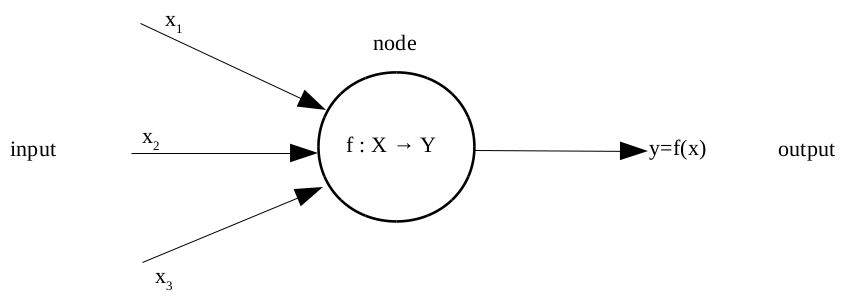
\includegraphics[width=10cm]{img/node}
\caption{}\label{fig1}
\end{figure}
\newline To gain an intuition of what a node is really doing, it's useful to get a more precise idea of a possible problem we could want to face with our node and of an appropriate map $f:X\rightarrow Y$ we might want to use.
\begin{Example}\label{example1}
Consider a given dataset $\{(x_i,y_i)\}$ like the one in the next picture, and suppose to have to find an appropriate relation in the form $y=f(x)$ in order to predict the value of the variable $y$, even for unknown $x$ which we might encounter in the future.
\begin{figure}[h]
	\centering
	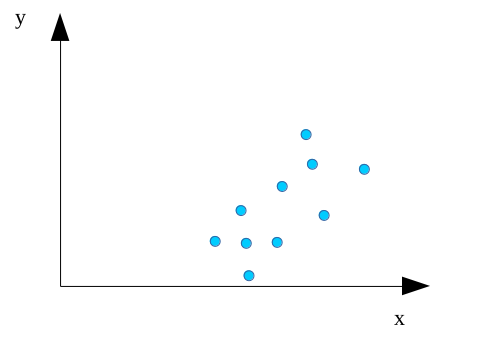
\includegraphics[width=7.5cm]{img/regression1}
	\caption{}
\end{figure}
\newline As widely known, linear regression can be a first good answer to the problem, so, once performed the calculations, we are able to write:
\[
y=wx + b
\]
for some $w,b$; let's call this linear transformation $L\!: \, Lx=wx+b$. Now suppose that the output $y$ has a constrain, e.g. that $y\ge0$ must hold\footnote{The reason why non linear function like the one arising from this constrain are needed in deep learning will be seen in the end of this section.} $ \forall y $. Then it would be reasonable to update the $f$ function as in the figure below:
\begin{figure}[h]
	\centering
	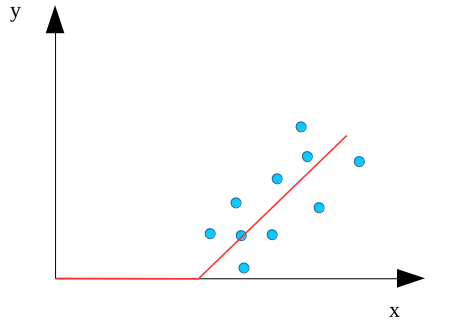
\includegraphics[width=7.5cm]{img/regression2} 
	\caption{}
\end{figure}
\newline Which mathematically means:
\[
y=max\{0,wx+b\}
\]
So we have that the response function $f$ is given by the composition of a linear function, $L$, and a non linear one, $A\,\,s.t.\,\, x\overset{A}{\longrightarrow}max\{0,x\}$, where of course every function is defined from $X$ to $Y$:
\[
f:X\rightarrow Y\quad s.t.\quad f=A\circ L
\]
In the deep learning literature the non linear function acting after the linear one is called \textit{Activation function}, while the specific one used in this example, namely $x\rightarrow max\{0,x\}$, is known as \textit{ReLU} function, which stands for \textit{Rectified Linear Unit}.$\qed$
\end{Example}
\noindent An approach like the one presented in example \ref{example1} unload all the complexity of a problem on the function $f$ that maps the given data to the predicted output; it thus become early less feasible as complexity grows. It's here that the neural network paradigm come in.\\
The main ideas behind it can be divided in two: a ``divide et impera''-like approach and a statistical-like one, based on random functions and optimization of appropriate functionals.\\
For what concerns the first, the idea is to stuck together different nodes in order to be able to reconstruct complex behaviors as the composition of simpler ones. This assembly of nodes is performed in two fashions: from one side we can imagine to feed in the data to different neurons, which will calculate their own output, and then to put together the outputs, building up what in the literature is called a \textit{layer} of nodes. From the other side we can put different layer in sequence, so that the first layer takes the input from the data, the second layer takes as input the output of the first one, and so on, until the last layer outputs the predicted y.\footnote{Technically it's more correct to say ``every node in the $n\!-\!th$ layer takes the input from every node in the $(n+1)\!-\!th$ layer'', but it's preferred to use the short sentence above when it's clear enough.}\\
Following the literature we call \textit{Hidden layer} every intermediate layer, as in the following picture.
\begin{figure}[h]
\centering
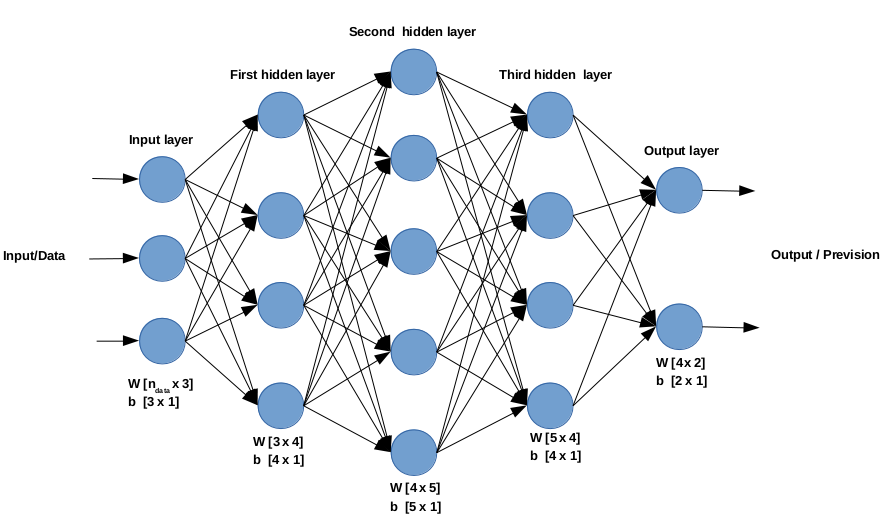
\includegraphics[width=0.95\textwidth]{img/neuralnet}
\caption{}\label{neuralnet}
\end{figure}
\newline
In deep learning the above mentioned process that brings the input to the output, passing by all the intermediate layers, is called \textit{forward propagation}, or, in short, forprop, and constitute the first part of the training algorithm of a neural network.\\
\newline \noindent One surprising aspect of neural networks is that they don't require their designer to decide which node of the first layer takes which part of the input, nor which nodes of the $n\!-\!th$ layer a generic node of the $(n+1)\!-\!th$ layer should consider, neither how much importance any node should give to each of its inputs. In fact, he gives all the inputs to every node, and let the neural network find it out by itself. In other words, given enough training example, i.e. enough $(x_i,y_i)$ known couples, neural networks are remarkably good at figuring out how to map unknown $x$ to the right $y$.\\
This capability is achieved by means of the second main idea of neural networks: what is called \textit{back propagation}, or backprop.\\
Let's consider again the single node as in figure \ref{fig1}, with $y=ReLU(wx+b)$. More precisely in this case we have:
\begin{equation}\label{linear}
L=\mathbf{w \cdot x} + b
\end{equation}
where $\mathbf x = (x_1,x_2,x_3)^T$, \textbf{w} is the vector of the \textit{weights}, since the dot product in \eqref{linear} can be seen as a weighted sum of the inputs, while \textit{b} is called \textit{bias}, since it affects this sum with a its contribution. \\
The basic idea is to perform a forward propagation with known data and randomly initialized parameters $\mathbf w,b$, then to calculate an appropriate distance between the predicted output, let's call it $\hat y$, and the known output\textit{y}.
This distance measure the \textit{cost C}, or the loss, of our computation.\\
Let's consider for simplicity:
\[
C=\frac{1}{2}(y-\hat y)^2
\]
Now we begin the backprop phase: we calculate the gradient of \textit{C} w.r.t. our parameters, and then we update them using an optimization algorithm aiming at minimizing the cost \textit{C}.\\
For example using gradient descent:
\begin{equation}\label{grad_desc}
\begin{cases}
\mathbf w \leftarrow \mathbf w - \alpha \frac{dC}{d\mathbf w} \\
b \,\,\leftarrow b\,\, - \,\,\alpha \frac{dC}{db}
\end{cases}
\end{equation}
where $\alpha$ is a, typically small, positive real number, which controls how fast we update our weights, and is thus called \textit{learning rate}.\\
The learning process is thus construct as a loop composed by forward propagation followed by backward propagation, with this sequence being repeated until the cost reaches a satisfying value.\\
Coming back to a full DNN, i.e. to a neural network with more than one hidden layer like the one in figure \ref{neuralnet}, it's easy to generalize the above algorithm.\\
Let's suppose we have a large enough dataset of $x_i$ with the corresponding $y_j$, and divided it in two disjoint subset, the \textit{training set} and the \textit{test set}.\\
We initialize all the weights randomly, and we start the loop, called \textit{training loop}, over the training set.\\
First we have forward propagation:
\begin{itemize}
\item every node of the input layer takes all the data as input, performs an affinity like the one in \eqref{linear} using it's own weights and bias, non-linearize the result through an activation function like the ReLU, and sends it's output to every node of the next layer;
\item every node of the hidden layers takes as input all the outputs coming from the previous layer, performs a weighted sum of them and adds a bias, using it's own parameters, and outputs the activated result to each node of the next layer;
\item the nodes in the last layer usually calculate only the linear transformation and outputs the predicted result.
\end{itemize}
At this point we calculate the value of the cost functional, and then we start backprop, in which every node, starting from the ones inside the last layer, calculate the gradients of the cost w.r.t. it's own parameters $w,b$ and updates them using an algorithm like gradient descent. Once we have updated all the parameters till the first layers we do another iteration of the algorithm.\\
When we are satisfied of the performance of our neural network, we do \textit{only one} forward propagation step, keeping the optimal parameters, but using the test set, and we evaluate the accuracy of the results.\\
\newline
\noindent Before going on with the discussion of deeper aspects of deep learning, we show why some of the choices made in the design of the neural network and of the algorithm are appropriate.\\
First of all it is important to notice that non linear activation function are in general necessary. In fact, consider a general DNN, identify with the subscript $l$ the quantities relative to the \textit{l}-th layer, call $n_d$ the number of the data in the set, $n_l$ the number of nodes in the layer l and suppose that $A$ is the identity for each node. We then have:
\[
A_l = L_l = W_l A_{l-1} + b_l
\]
where $A_{l}$ denotes the $n_l \times n_d$ matrix of the outputs of the \textit{l}-th layer, $W_l$ is a $n_{l-1} \times n_l $ matrix, and $b_l$ is a $n_l$ vector. Then we have:
\[
A_l=W_l(W_{l-1}A_{l-2} + b_{l-1})+ b_l = W_lW_{l-1}A_{l-2}+W_lb_{l-1}+b_l =: W'_l A_{l-2} +  b'_l
\]
By recursion is then easy to prove that in the end with a complete step of forward propagation we are computing only a linear combination of the initial data, as we would do in a much simpler way with just one node.\\
In this report we focus mainly on $tanh(\cdot)$ and ReLU activation functions, which are both very common choices, but others are being investigated as well.\\
For similar reasons it is very important to initialize the weights randomly: if we don't, and, for example, we initialize every parameter to a given value, then at the very first iteration all the nodes in the same layer are computing the very same output, and moreover are being updated at the same way during backward propagation. In the end this result in having a DNN that produces the same output of one which has just one node per layer.\\
Finally, it's worth noting that deep neural networks turn out to be more effective than bigger shallow neural networks in reconstructing and predicting complex behavior, especially when it is decomposable in a hierarchical grade of complexity, and that a minimum number of hidden layer is sometimes necessary. We don't prove it, but we will give a quantitative result of a comparison in section \ref{section2.2}, despite in a specific case.


\section{Further insights}\label{section1.2}


%%%%%%%%%%%%%%%%%%%%%%%%%%%%%%%%%%%%%%%%%%%%%%%%%%%%%%%%%%%%%%%%%%%%%%%%
%%%%%%%%%%%%%%%%%%%%%%%%%%%%%%%%%%%%%%%%%%%%%%%%%%%%%%%%%%%%%%%%%%%%%%%%


\chapter{Application to PDEs}\label{chapter2}

\section{The Poisson-Dirichlet problem}\label{section2.1}

\section{Some more in-depth theoretical results}\label{section2.2}


%%%%%%%%%%%%%%%%%%%%%%%%%%%%%%%%%%%%%%%%%%%%%%%%%%%%%%%%%%%%%%%%%%%%%%%%
%%%%%%%%%%%%%%%%%%%%%%%%%%%%%%%%%%%%%%%%%%%%%%%%%%%%%%%%%%%%%%%%%%%%%%%%


\chapter{Implementation of neural-net}\label{chapter3}
In this chapter an in-depth view of a Deep Learning C++ program, called \textit{neural-net}, is given.\\
The program has been built using the \cite{git} distributed version control system, with GitHub as hosting service, and can be freely cloned or downloaded from the author's page: \href{https://github.com/pjbaioni/neural-net}{\emph{https://github.com/pjbaioni/neural-net}}.\\
In order to build and run the program, some not included dependencies are needed, in particular a C++ compiler, \cite{make}, \cite{gnuplot}, \cite{eigen} and \cite{boost} libraries, while to build the documentation a TeX compiler has to be used; more details are given in the README.md file and in chapter \ref{chapter4}, where it is shown how to build the program and run an example. 

\section{Directory tree}
Downloading the repository ``neural-net'' one's find:
\begin{itemize}
	\item the \textit{data} folder, which contains the input and output data in .dat and .pot (for \cite{getpot}) format, \cite{gnuplot} scripts in .gnu format, and their graphical output in .png format;
	\item the \textit{doc} folder, containing this documentation in .tex and .pdf format, plus the \textit{img} sub-folder where there are the images included by the TeX file;
	\item the \textit{include} folder, containing the headers \textit{GetPot.hpp}, an utility used for parsing parameters file and command line option, \textit{gnuplot-iostream.hpp}, an utility used to output a graphical representation of the results in an interactive way, \textit{NeuralNetwork.hpp}, which holds the NeuralNetwork \textbf{class}, and \textit{Optimizers.hpp}, where all the optimizers employable from NeuralNetwork are defined as \textbf{class templates};
	\item the \textit{src} folder, which contain the source files main.cpp, NeuralNetwork.cpp, where the NeuralNetwork class member functions are defined, the Makefile which can be used to automatic build the main program, and the \textit{write\_set} sub-folder, where the \textit{write\_set.cpp} file used to generate datasets is placed;
	\item the COPYING file, a plain text file containing copying informations and licenses;
	\item the README.md file, a markdown file containing basic informations;
	\item the (hidden) \textit{.gitignore} file, that trace the file extensions which are not being pushed to the remote, mainly compilation files, executables and comments file.
\end{itemize}
\noindent Despite the different extensions, every non-png nor non-pdf file can be opened by any text editor.
\section{The Neural Network class}
\section{The Optimizers class templates}
\section{Write\_set and data}
\section{The main}

%%%%%%%%%%%%%%%%%%%%%%%%%%%%%%%%%%%%%%%%%%%%%%%%%%%%%%%%%%%%%%%%%%%%%%%%
%%%%%%%%%%%%%%%%%%%%%%%%%%%%%%%%%%%%%%%%%%%%%%%%%%%%%%%%%%%%%%%%%%%%%%%%


\chapter{Examples}\label{chapter4}

\section{Building instructions}
\section{Reconstruction of a wave packet}

%%%%%%%%%%%%%%%%%%%%%%%%%%%%%%%%%%%%%%%%%%%%%%%%%%%%%%%%%%%%%%%%%%%%%%%%
%%%%%%%%%%%%%%%%%%%%%%%%%%%%%%%%%%%%%%%%%%%%%%%%%%%%%%%%%%%%%%%%%%%%%%%%


\chapter*{Conclusions and further developments}
\addcontentsline{toc}{chapter}{Conclusions and further developments}


%%%%%%%%%%%%%%%%%%%%%%%%%%%%%%%%%%%%%%%%%%%%%%%%%%%%%%%%%%%%%%%%%%%%%%%%
%%%%%%%%%%%%%%%%%%%%%%%%%%%%%%%%%%%%%%%%%%%%%%%%%%%%%%%%%%%%%%%%%%%%%%%%


\appendix
\chapter*{Appendix}\label{appendix}
\addcontentsline{toc}{chapter}{Appendix}


%%%%%%%%%%%%%%%%%%%%%%%%%%%%%%%%%%%%%%%%%%%%%%%%%%%%%%%%%%%%%%%%%%%%%%%%
%%%%%%%%%%%%%%%%%%%%%%%%%%%%%%%%%%%%%%%%%%%%%%%%%%%%%%%%%%%%%%%%%%%%%%%%


\newpage
\begin{thebibliography}{10}
	\addcontentsline{toc}{chapter}{Bibliography}
	
	\bibitem[APSC]{PACS} Advanced Programming for Scientific Computing course lectures, Politecnico di Milano, 2019.
	\bibitem[Andrew NG]{AndrewNG} Professor Andrew NG's Deep Learning MOOC at Coursera, \href{https://www.coursera.org/specializations/deep-learning}{\emph{https://www.coursera.org/specializations/deep-learning}}, consulted in 2019.
	\bibitem[Boost]{boost} Boost C++ libraries, \href{https://www.boost.org/}{\emph{https://www.boost.org/}}
	\bibitem[cppreference.com]{cppreference} An online reference of the C++ language, \href{https://en.cppreference.com/w/cpp}{\emph{https://en.cppreference.com/w/cpp}}
	\bibitem[Eigen]{eigen} Eigen C++ template library for linear algebra, \href{https://eigen.tuxfamily.org/}{\emph{https://eigen.tuxfamily.org/}}
	\bibitem[FreeFem++]{freefem++} FreeFem++ PDE solver, \href{https://freefem.org/}{\emph{https://freefem.org/}}
	\bibitem[GetPot]{getpot} GetPot command line parser, \href{http://getpot.sourceforge.net/}{\emph{http://getpot.sourceforge.net/}}
	\bibitem[Git]{git} Git distributed version control system, \href{https://git-scm.com/}{\emph{https://git-scm.com/}}
	\bibitem[gnuplot]{gnuplot} A GNU graphing utility, \href{http://www.gnuplot.info/}{\emph{http://www.gnuplot.info/}}
	\bibitem[gnuplot-iostream]{gnuplot-iostream} A C++ interface to gnuplot, \href{https://github.com/dstahlke/gnuplot-iostream}{\emph{https://github.com/dstahlke/gnuplot-iostream}}
	\bibitem[Jinchao Xu et al.]{Jinchao} Juncai He, Lin li, Jinchao Xu, Chunyue Zheng, \emph{ReLU Deep Neural Networks and Linear Finite Elements}, 2018, found at \href{https://arxiv.org/abs/1807.03973}{\emph{https://arxiv.org/abs/1807.03973}}
	\bibitem[Kailai et al.]{Kailai} Kailai Xu, Bella Shi, Shuyi Yin, code and technical report of the project for the course CS230 \emph{Deep Learning, Winter 2018, Stanford University}, found at \href{https://github.com/kailaix/nnpde}{\emph{https://github.com/kailaix/nnpde}}
	\bibitem[Kingma-LeiBa]{Kingma} Diederik P. Kingma, Jimmy Lei Ba,\emph{Adam: a method for stochastic optimization}, 2015, found at
	\href{https://arxiv.org/abs/1412.6980}{\emph{https://arxiv.org/abs/1412.6980}} 
	\bibitem[Make]{make} GNU Make doc at \href{https://www.gnu.org/software/make/manual}{\emph{https://www.gnu.org/software/make/manual}}
	\bibitem[Weinan-Bing]{Weinan} Weinan E, Bing Yu \emph{The Deep Ritz method: A deep learning-based numerical algorithm for solving variational problems}, 2017, found at \href{https://arxiv.org/abs/1710.00211}{\emph{https://arxiv.org/abs/1710.00211}}
	
\end{thebibliography}


\end{document}	
